\documentclass[12pt,a4paper,italian]{book}

% numera i subsubsection 1 - 1.1 - 1.1.1 - 1.1.1.1
\setcounter{secnumdepth}{3}

%%%%%%%%%%%%%%%%%%%%%%%%%%%%%%%%%%%%%%
%    Scelta dei package da usare     %
%%%%%%%%%%%%%%%%%%%%%%%%%%%%%%%%%%%%%%
\usepackage[italian]{babel}
\usepackage[utf8]{inputenc}
\usepackage[T1]{fontenc}
\usepackage{amsmath,amsfonts,amssymb,amsthm}
\usepackage{deistesi}
\usepackage{fancyhdr}
\usepackage{multirow}
\usepackage{tabularx}
\usepackage{float}
\usepackage[final]{listings}
\usepackage[pdftex,dvipsnames]{xcolor}
\usepackage{inconsolata}
\usepackage{xargs}
\usepackage[colorinlistoftodos,prependcaption]{todonotes}
\usepackage{rotating}

\usepackage[
   pdftex,
   pdfauthor={Luca Pascucci},
   pdftitle={Synapsis - Middleware per l'integrazione di Game Engine e Sistemi Multi-Agente},
   pdfsubject={Tesi Laurea magistrale},
   pdfkeywords={Sistema Multi-Agente, Game Engine, Middleware, Play framework, Ambiente virtuale},
   bookmarks=true,
   bookmarksopen=true,
   breaklinks=true,
   colorlinks=true,
   linkcolor=black,
   anchorcolor=blue,
   citecolor=blue,
   filecolor=red,
   urlcolor=blue,
   pdfborderstyle={/S/U/W 1} % border style will be underline of width 1pt
]{hyperref}

\urlstyle{same}

\definecolor{mygray}{gray}{0.6}
\definecolor{delim}{RGB}{20,105,176}
\colorlet{myred}{red!60!black}
\colorlet{numb}{red!60!black}

\lstset{
   frame=bt,
   captionpos=b,
   aboveskip=3mm,
   belowskip=3mm,
   showspaces=false, % show spaces everywhere adding particular underscores; it overrides 'showstringspaces'
   showstringspaces=false, % underline spaces within strings only
   showtabs=false,
   columns=flexible,
   extendedchars=true,
   basicstyle=\fontsize{10}{10}\ttfamily,
   numbers=left,
   stepnumber=3,
   numberstyle=\tiny\color{gray},
   keywordstyle=\color{blue},
   commentstyle=\color{ForestGreen},
   stringstyle=\color{mygray},
   breaklines=true,
   breakatwhitespace=true,
   tabsize=2,
   title=\lstname,
   literate=
  {á}{{\'a}}1 {é}{{\'e}}1 {í}{{\'i}}1 {ó}{{\'o}}1 {ú}{{\'u}}1
  {Á}{{\'A}}1 {É}{{\'E}}1 {Í}{{\'I}}1 {Ó}{{\'O}}1 {Ú}{{\'U}}1
  {à}{{\`a}}1 {è}{{\`e}}1 {ì}{{\`i}}1 {ò}{{\`o}}1 {ù}{{\`u}}1
  {À}{{\`A}}1 {È}{{\'E}}1 {Ì}{{\`I}}1 {Ò}{{\`O}}1 {Ù}{{\`U}}1
  {ä}{{\"a}}1 {ë}{{\"e}}1 {ï}{{\"i}}1 {ö}{{\"o}}1 {ü}{{\"u}}1
  {Ä}{{\"A}}1 {Ë}{{\"E}}1 {Ï}{{\"I}}1 {Ö}{{\"O}}1 {Ü}{{\"U}}1
  {â}{{\^a}}1 {ê}{{\^e}}1 {î}{{\^i}}1 {ô}{{\^o}}1 {û}{{\^u}}1
  {Â}{{\^A}}1 {Ê}{{\^E}}1 {Î}{{\^I}}1 {Ô}{{\^O}}1 {Û}{{\^U}}1
  {Ã}{{\~A}}1 {ã}{{\~a}}1 {Õ}{{\~O}}1 {õ}{{\~o}}1
  {œ}{{\oe}}1 {Œ}{{\OE}}1 {æ}{{\ae}}1 {Æ}{{\AE}}1 {ß}{{\ss}}1
  {ű}{{\H{u}}}1 {Ű}{{\H{U}}}1 {ő}{{\H{o}}}1 {Ő}{{\H{O}}}1
  {ç}{{\c c}}1 {Ç}{{\c C}}1 {ø}{{\o}}1 {å}{{\r a}}1 {Å}{{\r A}}1
  {€}{{\euro}}1 {£}{{\pounds}}1 {«}{{\guillemotleft}}1
  {»}{{\guillemotright}}1 {ñ}{{\~n}}1 {Ñ}{{\~N}}1 {¿}{{?`}}1
}

\lstset{
  language=Java,
  morekeywords={final}
  moredelim=[il][\textcolor{mygray}]{@}{\ },
  moredelim=[is][\textcolor{mygray}]{\%\%}{\%\%}
}

\lstdefinelanguage{json}{
    comment=[l]{//},
    literate=
      {0}{{{\color{myred}0}}}{1}
      {1}{{{\color{myred}1}}}{1}
      {2}{{{\color{myred}2}}}{1}
      {3}{{{\color{myred}3}}}{1}
      {4}{{{\color{myred}4}}}{1}
      {5}{{{\color{myred}5}}}{1}
      {6}{{{\color{myred}6}}}{1}
      {7}{{{\color{myred}7}}}{1}
      {8}{{{\color{myred}8}}}{1}
      {9}{{{\color{myred}9}}}{1}
      {:}{{{\color{myred}{:}}}}{1}
      {,}{{{\color{myred}{,}}}}{1}
      {\{}{{{\color{delim}{\{}}}}{1}
      {\}}{{{\color{delim}{\}}}}}{1}
      {[}{{{\color{delim}{[}}}}{1}
      {]}{{{\color{delim}{]}}}}{1},
}

\lstdefinelanguage{asl}{
    comment=[l]{//},
    morestring=**[d][\color{myred}]{"},
    keywords={include}
}


\newcommandx{\unsure}[2][1=]{\todo[linecolor=red,backgroundcolor=red!25,bordercolor=red,#1]{#2}}
\newcommandx{\change}[2][1=]{\todo[linecolor=blue,backgroundcolor=blue!25,bordercolor=blue,#1]{#2}}
\newcommandx{\improvement}[2][1=]{\todo[linecolor=ForestGreen,backgroundcolor=ForestGreen!25,bordercolor=ForestGreen,#1]{#2}}
\newcommandx{\marianiSays}[2][1=]{\todo[linecolor=Orange,backgroundcolor=Orange!25,bordercolor=Orange,#1]{#2}}

\makeatletter

\newcommand\ProcessThreeDashes{\llap{\color{cyan}\mdseries-{-}-}}

%%%%%%%%%%%%%%%%%%%%%%%%%%%%%%%%%%%%%%%%
% Scelta delle dimensioni della pagina %
%%%%%%%%%%%%%%%%%%%%%%%%%%%%%%%%%%%%%%%%

\setlength{\textwidth}{13.5cm}
\setlength{\textheight}{19cm}
\setlength{\footskip}{3cm}
\setlength{\headheight}{15pt}
\oddsidemargin=50pt \evensidemargin=20pt

%%%%%%%%%%%%%%%%%%%%%%%%%%%%%%%%%%%%%%
%  Informazioni generali sulla Tesi  %
%    da usare nell'intestazione      %
%%%%%%%%%%%%%%%%%%%%%%%%%%%%%%%%%%%%%%

\titolo{Synapsis - Middleware per l'integrazione di Game Engine e Sistemi Multi-Agente}
\laureando{Luca Pascucci}
\annoaccademico{2018--2019}
\sessione{II}
\facolta{CAMPUS DI CESENA\\SCUOLA DI INGEGNERIA E ARCHITETTURA}
\corsodilaurea{Ingegneria e Scienze Informatiche}
\corso{Sistemi Autonomi}
\relatore{Andrea Omicini}
\correlatorea{Stefano Mariani}
\parolechiave{Sistema Multi-Agente}{Game Engine}{Middleware}{Play Framework}{Ambiente virtuale}

\dedica{\textit{"Dedico questo mio lavoro che si pone a conclusione di un lungo e gioioso cammino alle persone che mi hanno aiutato ed insegnato"}}

\author{Luca Pascucci}
\title{Synapsis - Middleware per l'integrazione di Game Engine e Sistemi Multi-Agente}
\date{\today}

%%%%%%%%%%%%%%%%%%%%%%%%%%%%%%%%%%%%%
% Fine Preambolo %
% Inizio tesi %
%%%%%%%%%%%%%%%%%%%%%%%%%%%%%%%%%%%%%%

\begin{document}

%%%%%%%%%%%%%%%%%%%%%%%%%
% inizio prefazione
% pagina del titolo, indice, sommario
%%%%%%%%%%%%%%%%%%%%%%%%%

\frontmatter \maketitle \pagestyle{plain} \tableofcontents


\chapter{Introduzione}

L'ambiente, per definizione, è tutto ciò che circonda e con cui interagisce un organismo \cite{treccani}. I Sistemi Multi-Agente (MAS) forniscono diverse astrazioni per la costruzione di un sistema software, ma le tecnologie disponibili risultano spesso carenti sotto il punto di vista della costruzione dell'ambiente (virtuale) in cui gli agenti operano, poiché si concentrano solamente sulla definizione di un ambiente computazionale esclusivamente logico, slegato dal mondo fisico (che può invece essere rappresentato sul piano virtuale). 

\medskip

Le Game Engine (GE), ovvero framework utilizzati per supportare la progettazione e lo sviluppo di videogiochi, viceversa, sono sempre più spesso utilizzate al di fuori dell'ambito video-ludico per rappresentare e gestire ambienti (virtuali) complessi, potenzialmente riflesso di un ambiente fisico, ad esempio in scenari di simulazione tattica (militare, di soccorso, etc.). In particolare, di recente le GE sono state utilizzate come mezzo abilitante per la coordinazione \cite{gamemas-woa2016} all'interno di MAS.

\medskip 

L'ambiente, o scena, secondo la terminologia dei videogiochi, è una parte fondamentale che permette al giocatore di entrare in sinergia con il tipo, lo scopo e le modalità del gioco. Un esempio lampante è un FPS\footnote{First-Person Shooter = sparatutto in prima persona} dove la scena è solitamente vista in prima persona dal videogiocatore, e la presenza di elementi con i quali interagire, crea interesse nel giocatore ad esplorare l'ambiente attorno a lui.

\medskip

In questa tesi si intende studiare lo stato di integrazione tra Game Engine (GE) e Sistemi Multi-Agente (MAS), per proporre un'infrastruttura generica utilizzabile per diversi scenari di associazione e comunicazione tra MAS e GE rispettandone il disaccoppiamento e l'integrità concettuale delle loro astrazioni.

\medskip

Il primo capitolo introduce il lettore ai Sistemi Multi-Agente (MAS), alle Game Engine (GE) ed alle integrazioni già realizzate in passato. Vengono dunque illustrate le astrazioni presenti nei MAS, le GE e si studia lo stato dell'arte delle integrazioni.

\medskip

Il secondo capitolo, poi, analizza i differenti modelli computazionali delle tecnologie utilizzate, al fine di definire delle linee guida all'integrazione dei due sistemi, e descrive la struttura del sistema di integrazione.

\medskip

Il terzo capitolo contiene una descrizione più approfondita degli elementi che compongono il middleware, la tecnologia di comunicazione utilizzata per collegare le diverse parti del sistema e le librerie sviluppate per mettere in comunicazione MAS e GE attraverso il middleware.

\medskip

Il quarto capitolo contiene il caso di studio preso in esame per convalidare il sistema precedentemente delineato, mostrando struttura dei componenti realizzati e illustrando il flusso di interazione tra essi. Infine, nel Capitolo 5 si discuterà circa le conclusioni e verranno forniti spunti di riflessione per eventuali lavori futuri.

\medskip

La principale motivazione che ha portato a questo studio risiede nel fatto che seppur la ricerca sui MAS ha prodotto modelli ricchi di astrazioni anche per la modellazione della dimensione ambientale, oltre a quella agentesca e sociale, le tecnologie che dovrebbero reificare tali modelli sono più rare e spesso limitate. Uno degli esempi più ricchi è costituito dal framework CArtAgO \cite{cartago}, non a caso sfruttato per il design e l'implementazione dell'infrastruttura proposta in questa tesi.

\medskip

Esiste un divario nel progresso tecnologico che le GE hanno raggiunto rispetto al livello tecnologico delle infrastrutture orientate agli agenti nate all'interno della comunità accademica. Ciò non dovrebbe sorprendere nessuno: il settore video-ludico può contare su un maggiore supporto economico e su milioni di sviluppatori e tester (oltre ai giocatori), che sono ben pagati per spingere stabilità, prestazioni, usabilità dei loro prodotti a livelli di qualità senza precedenti e senza pari. Pertanto, vale la pena considerare la possibilità di trarre vantaggio da tali prodotti finemente ottimizzati per migliorare la qualità delle tecnologie mirate alla rappresentazione e gestione di ambienti virtuali nei MAS \cite{ge-architecture}.

\medskip

Una integrazione MAS -- GE non darebbe benefici solo la "mondo MAS". C'è una lacuna nelle astrazioni concettuali e progettuali che la GE fornisce agli sviluppatori rispetto alle astrazioni molto più ricche che offrono soluzioni di ingegneria del software orientate agli agenti. La GE presa in considerazione in questo documento, Unity \cite{unity}, ad esempio fornisce astrazioni di livello molto basso, specialmente lato "personaggi attivi", dove, ad esempio, programmare un comportamento ciclico e orientato a un goal equivale a scrivere coroutine che attraversano più fasi di rendering---goal e piani per raggiungerli non sono modellati da astrazioni di prima classe. 

\medskip

Inoltre, l'integrazione di MAS con GE può fornire nuove soluzioni per affrontare le problematiche tipiche degli scenari di realtà aumentata in cui si richiede che l'agente sia consapevole dello spazio in un ambiente fisico, sfruttando le tecnologie a disposizione nelle GE. D'altro canto tale integrazione mette a disposizione nuove funzionalità in grado di realizzare, all'interno dell'ecosistema GE, oggetti autonomi come ad esempio gli NPC\footnote{Non-Player Character: è un personaggio che non è sotto il controllo diretto del giocatore, ma viene invece gestito dal game master o dalla IA del software nel caso dei videogiochi} utilizzando le astrazioni presenti nei MAS.

%%%%%%%%%%%%%%%%%%%%%%%%%
% inizio corpo del documento
% sequenze dei vari capitoli
% è consigliato mantenere una struttura logica ben definita per separare i vari capitoli
% si consiglia di reificare tale struttura fisicamente sul file system
%%%%%%%%%%%%%%%%%%%%%%%%%

\mainmatter

% stile della pagina
\pagestyle{fancy} \fancyhead[LE,RO]{\bfseries\thepage}

% inclusione dei capitoli

\chapter{Background}

\subsection{Integrazione}

Sono già presenti esempi di integrazione tra GE e MAS che concentrano la propria attenzione su obiettivi specifici a livello tecnologico, piuttosto che sulla creazione di un'infrastruttura orientata agli agenti basata sul gioco per scopi generici. Per esempio:

\begin{itemize}
    \item QuizMASter \cite{5763564} concentrato sull'astrazione degli agenti collegando gli agenti MAS ai personaggi dei motori di gioco, nel contesto dell'apprendimento educativo
    \item CIGA \cite{ciga} considera sia la modellazione degli agenti che quella dell'ambiente, per agenti virtuali generici in ambienti virtuali
    \item GameBots \cite{gamebots} concentrato sull'astrazione dell'agente, ma considera anche l'ambiente fornendo un framework di sviluppo e un runtime per i test di sistemi multi-agente in ambienti virtuali
    \item UTSAF \cite{utsaf} si concentra sulla modellistica ambientale nel contesto di simulazioni distribuite in ambito militare\footnote{Gli agenti vengono considerati, ma solo come mezzo di integrazione tra diverse piattaforme di simulazione, non nel contesto del GE sfruttato per il rendering di simulazione}
\end{itemize}

Sebbene rappresentino chiaramente esempi di integrazione (parzialmente) riuscita di MAS in GE, i lavori sopra elencati presentano alcune carenze rispetto all'obiettivo che perseguiamo in questo documento.

\smallskip

Solamente CIGA rappresenta un'eccezione che riconosce il divario concettuale tra MAS e GE, e propone soluzioni per affrontarlo (anche se a livello tecnologico). L'unico strato preso in considerazione nel perseguimento dell'integrazione è quello tecnologico - nessun modello, nessuna architettura, nessun linguaggio. All'interno di QuizMASter, UTSAF e GameBot (in una certa misura) l'integrazione è realizzata per specifico obiettivo, e la maggior parte degli approcci fornisce ai programmatori alcune astrazioni per trattare con agenti e ambiente, ma nessuna attenzione viene data alle astrazioni sociali \cite{gamemas-woa2016}.


\section{Situazione iniziale}

I lavori precedentemente svolti, che hanno contribuito alla definizione di questo percorso, utilizzano due approcci nettamente separati per l'integrazione MAS e GE:
\begin{enumerate}
	\item Integrazione delle caratteristiche dei MAS all'interno della GE;
	\item Realizzazione di un middleware, come layer software, per collegare l'ambiente MAS con GE.
\end{enumerate}

\subsection{MAS all'interno di GE} \label{MAS_dentro_GE}

Il primo punto è stato realizzato implementando due modelli tipici dei MAS:
\begin{itemize}
	\item Il modello Beliefs, Desires, Intentions (BDI) per la programmazione degli agenti \cite{amslaurea15657};
	\item Un modello di coordinazione degli agenti tramite spazio di tuple e primitive Linda \cite{amslaurea8424}\cite{amslaurea16100};
\end{itemize}

Il cuore pulsante di entrambi i lavori risiede nell'uso intensivo di un interprete Prolog fatto ad hoc per Unity: UnityProlog \cite{unity_prolog}. Questo interprete dispone di molte funzionalità per estendere l'interoperabilità di Prolog con i GameObject.
Dal momento che è stato progettato per essere usato in maniera specifica con Unity, nasce con delle primitive che permettono di accedere e manipolare GameObject e i relativi componenti direttamente da Prolog. UnityProlog introduce tuttavia alcune limitazioni da tenere bene in considerazione \cite{amslaurea15657}, anche se allo stato attuale è l'unica versione di Prolog del quale è stato dimostrato il corretto funzionamento:
\begin{itemize}
	\item Un interprete per Prolog non sarà mai performante quanto lo può essere un compilatore e questo può rappresentare un problema per simulazioni di MAS piu grandi.
	\item Utilizza lo stack C\# come stack di esecuzione, quindi la tail call optimization non è ancora supportata.
	\item Non supporta regole con più di 10 subgoal, quindi a fronte di una regola complessa con tanti goal da controllare, è necessario frammentare la regola in questione in sotto regole con non più di 10 subgoal per ognuna.
\end{itemize}

\subsection{MAS e GE separati} \label{MAS_GE_separati}

Il secondo percorso si differenzia dal primo per la scelta di lasciare separati GE da MAS realizzando un canale di comunicazione tra i due ambienti. \'E stata introdotta una terminologia per contraddistinguere le entità realizzate sul GE (GameObject) e su MAS (agenti), rispettivamente definite "corpi" e "menti" virtuali. \cite{amslaurea12270}

\medskip

Fondamentalmente un corpo deve eseguire azioni e a seguito di determinati eventi deve trasmettere le proprie percezioni alla mente, mentre la mente deve elaborare le percezioni per decidere quali azioni deve far svolgere al proprio corpo. Per rendere possibile questa comunicazione è stato progettato e implementato un sistema middleware definito secondo il seguente schema.

\begin{figure}[H]
\centering
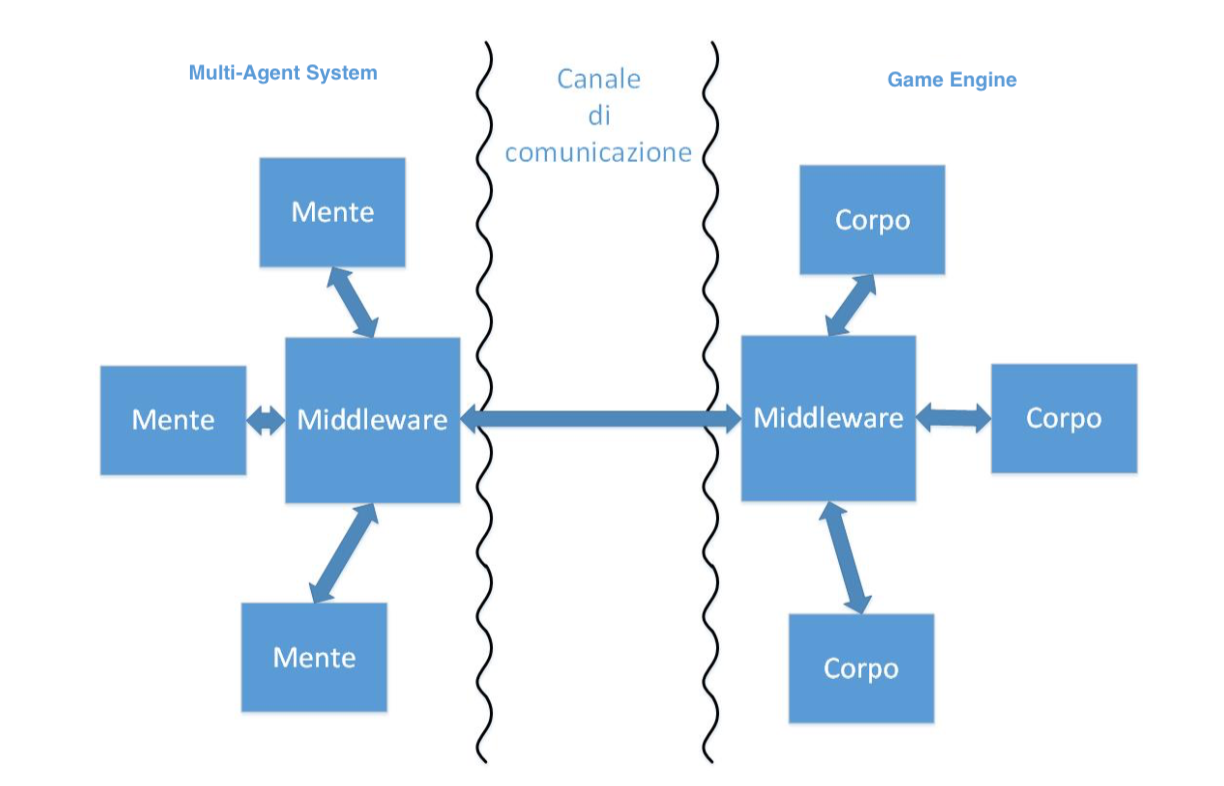
\includegraphics[width=9cm]{figures/Middleware_fuschini.png}
\caption{Il middleware viene suddiviso in due parti, poste sui due lati del canale di comunicazione. \cite{amslaurea12270}}
\end{figure}

Dallo schema si può notare la separazione del middleware nei due sistemi, motivato dalle diverse tecnologie utilizzate dai due ambienti.
Questa divisione vincola la realizzazione di una nuova parte di middleware in caso di utilizzo di un diversa tipologia di GE e/o MAS.
\medskip

Il protocollo di comunicazione tra le entità è stato realizzato utilizzando messaggi strutturati. Da una parte, le menti devono definire quale azione deve compiere il relativo corpo (es. "muoviti in avanti", "ruota", "prendi", ecc.), dall'altro i corpi devono far sapere alle relative menti le proprie percezioni dell'ambiente circostante (es. "mi ha toccato un'entità", "sono alle coordinate 23,12,-6", ecc.).\cite{amslaurea12270}


\subsection{JaCaMo}

JaCaMo è un framework per la programmazione orientata agli agenti che combina tre tecnologie già affermate e sviluppate da diversi anni.

\medskip

Un sistema multi-agente JaCaMo o, equivalentemente, un sistema software programmato con JaCaMo è definito da un'organizzazione Moise di agenti BDI autonomi basati su concetti come ruoli, gruppi, missione e schemi, implementati tramite Jason, che lavorano in ambienti condivisi distribuiti basati su artefatti, programmati in CArtAgO.

\medskip

Ognuna delle tre tecnologie indipendenti che compongono il framework ha il proprio set di astrazioni, modelli di programmazione e meta-modelli di riferimento, per questo motivo in JaCaMo è stato realizzato un meta-modello globale, con l'obiettivo di definire le dipendenze, connessioni, mapping concettuali e le sinergie tra le differenti astrazioni rese disponibili da ogni livello \cite{BOISSIER2013747}.

\begin{figure}[H]
\centering
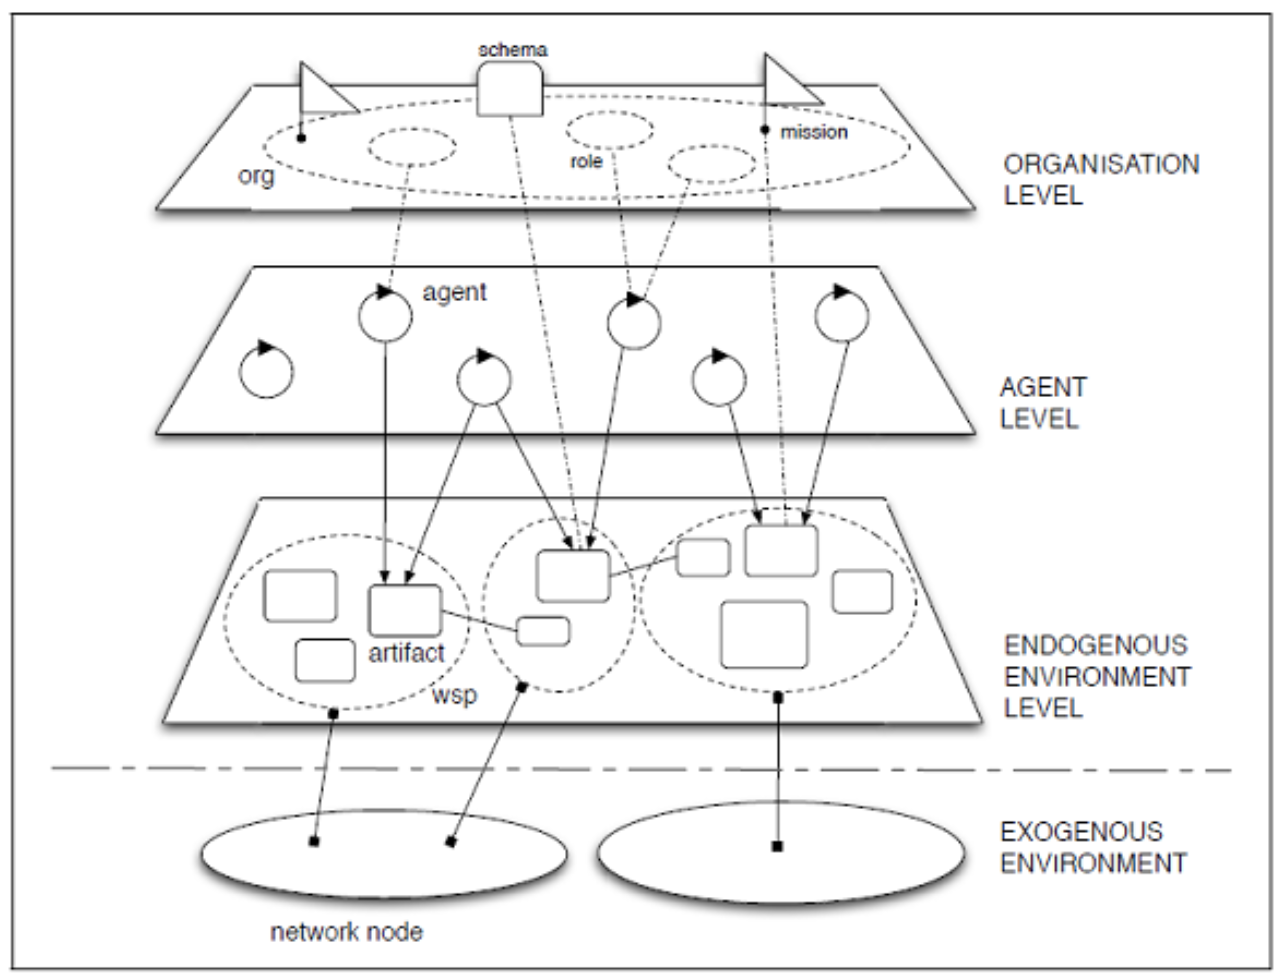
\includegraphics[width=\textwidth]{figures/JaCaMo_levels.png}
\caption{Livelli che compongono il framework JaCaMo \cite{BOISSIER2013747}}
\label{livelli_jacamo}
\end{figure}

\subsubsection{Jason} \label{jason}

Jason è un interprete di AgentSpeak che implementa la semantica operazionale del linguaggio e fornisce una piattaforma di sviluppo per Sistemi Multi-Agente, con molte funzionalità personalizzabili dall'utente.

\medskip

Le astrazioni appartenenti alla dimensione degli agenti, correlate al meta-modello Jason, sono principalmente ispirate all'architettura BDI sulla quale Jason è radicato. Quindi un agente è un'entità composta da un insieme di "beliefs", che rappresenta lo stato corrente e la conoscenza dell'agente sull'ambiente in cui si trova, una serie di "goals", che corrispondono a compiti che l'agente deve perseguire e una serie di "plans" ossia sequenze di azioni (external action or internal action), innescate da eventi, che gli agenti possono comporre, istanziare ed eseguire dinamicamente per compiere i "goals" \cite{jason-book}.

\subsubsection{CArtAgo}
Per quanto riguarda l'ambiente, ciascuna istanza dell'ambiente CArtAgO\footnote{Common ARTifact infrastructure for AGents Open environments} è composta da una o più entità workspace. Ogni workspace è formato da un insieme di artefatti, che forniscono un insieme di operazioni e proprietà osservabili, definendo anche l'interfaccia di utilizzo degli artefatti. L'esecuzione dell'operazione potrebbe generare aggiornamenti delle proprietà osservabili e degli eventi osservabili specifici. L'ultima entità relativa all'ambiente è il “manual”, un'entità utilizzata per descrivere le funzionalità fornite da un artefatto.
Cartago è basato sul meta-modello A\&A (Agents \& Artifacts), che definisce gli agenti come entità computazionali che compiono qualche tipo di attività che mira a uno scopo e gli artefatti come risorse e strumenti costruiti dinamicamente, usati e manipolati dagli agenti per supportare/realizzare le loro attività \cite{cartago}.

\smallskip

\paragraph{Artefatto}
L'artefatto è un'entità reattiva, non autonoma, stateful, riutilizzabile, controllabile ed osservabile. Modellano strumenti, risorse e porzioni di ambiente agendo da strumenti mediatori di azioni e interazioni sociali tra partecipanti individuali e lo stesso ambiente \cite{Omicini2008}.

\begin{figure}[H]
\centering
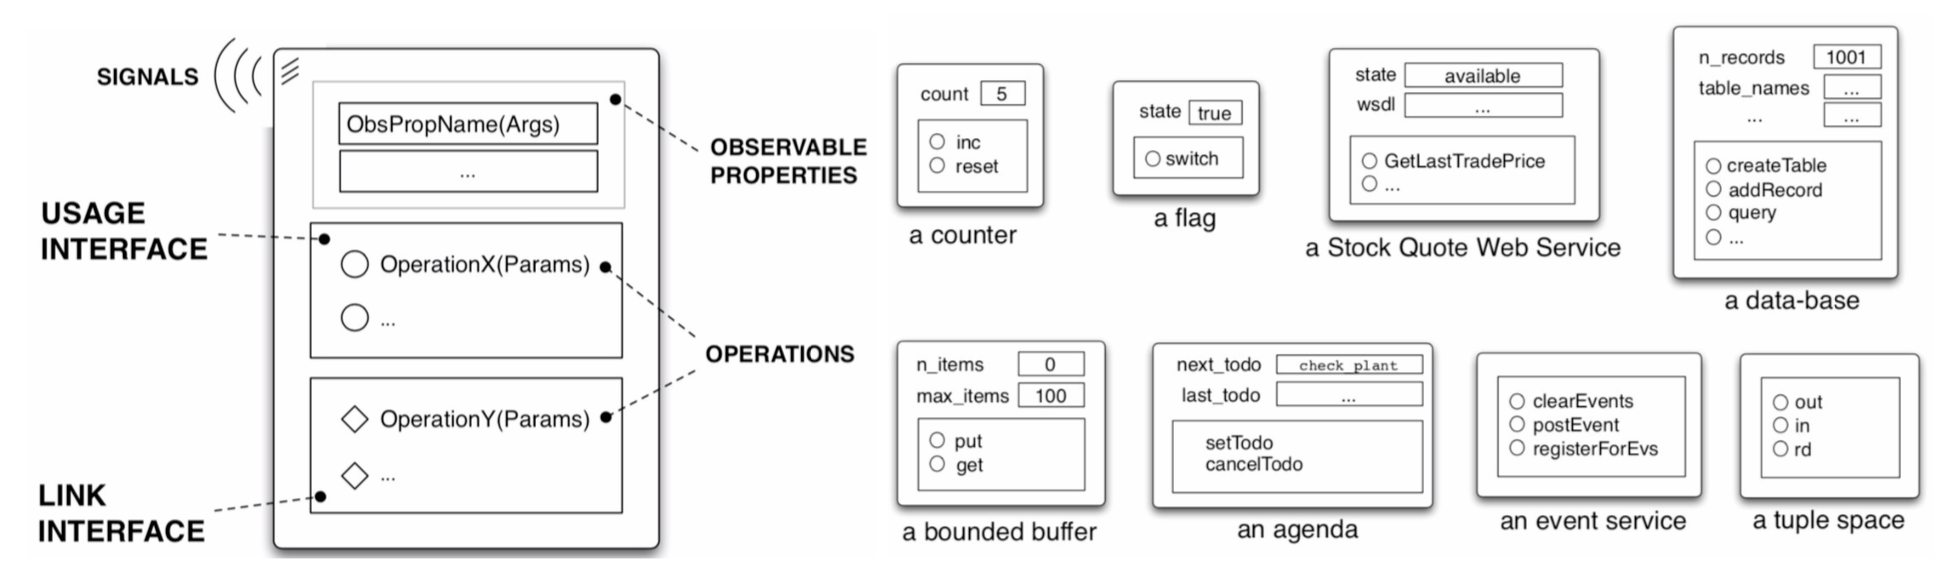
\includegraphics[width=\linewidth]{figures/Artifact_structure_example.png}
\caption{Struttura artefatto con relativi esempi}
\end{figure}

La modalità di interazione tra artefatto ed agente viene riepilogato nell'immagine sottostante.

\begin{figure}[H]
\centering
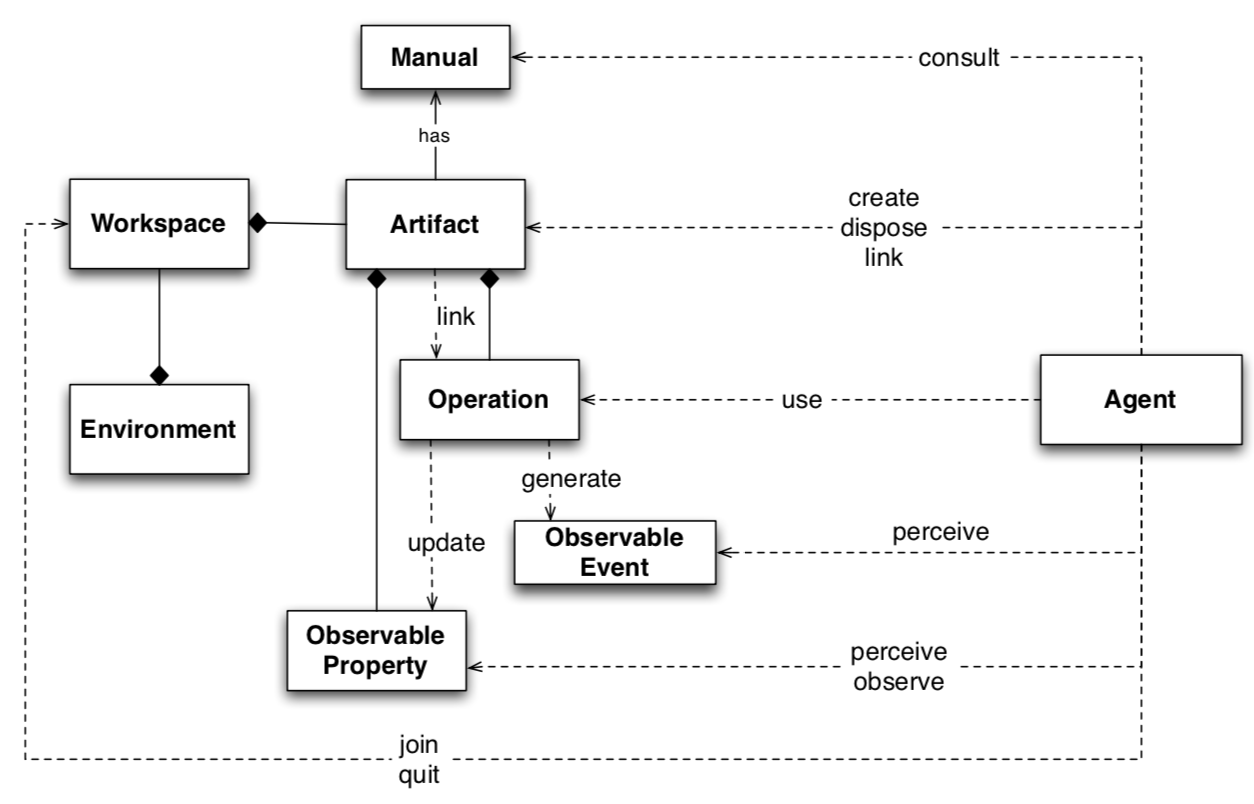
\includegraphics[width=\linewidth]{figures/Artifact_Agent_interaction.png}
\caption{Interazione tra agente ed artefatto}
\end{figure}

\subsubsection{Moise}
Moise è un meta-modello organizzativo per MAS basato sulle nozioni di ruoli, gruppi e missioni. Abilita un MAS ad avere specifiche esplicite per la sua organizzazione. Queste specifiche sono usate sia dagli agenti per ragioni inerenti la loro organizzazione, sia da una piattaforma organizzativa che si assicuri che gli agenti seguano le specifiche.

Moise permette di definire una gerarchia di ruoli con autorizzazioni e missioni, da assegnare agli agenti. Questo permette ai sistemi con un'organizzazione forte, di guadagnare proprietà di apertura (essenzialmente, la proprietà di lavorare con un numero e una diversità di componenti che non è imposta una volta per tutte) e adattamento.



\chapter{Synapsis: Modello e architettura}

In questo capitolo viene definita la terminologia usata nella restante parte della trattazione, vengono analizzati i differenti modelli computazionali delle tecnologie utilizzate per definire delle linee guida di integrazione dei sistemi e infine viene spiegata la struttura del sistema di integrazione.

\section{Terminologia}

La sinapsi (o giunzione sinaptica) (dal greco synàptein, vale a dire "connettere") è una struttura altamente specializzata che consente la comunicazione delle cellule del tessuto nervoso tra loro (neuroni) o con altre cellule (cellule muscolari, sensoriali). Nello specifico la sinapsi neuromuscolare rappresenta la giunzione tra neurone motore e muscolo a livello della placca motrice, ove ha luogo la trasmissione dell'impulso con le modalità delle sinapsi chimiche: lo spazio extracellulare della sinapsi neuromuscolare è detto chiave sinaptica \cite{treccani}.
La semplice associazione tra l'obiettivo di questo percorso e la parola sopra definita ha portato a denominare il middleware "Synapsis"\footnote{Traduzione in inglese del termine italiano sinapsi.}.

\subsection{Entità}

Successivamente nella trattazione verrà fatto uso del termine "entità" che generalmente viene intesa come insieme di elementi dotati di proprietà comuni dal punto di vista dell’applicazione considerata \cite{treccani}.
Concettualmente, in questo dominio, l'entità viene intesa come oggetto divisibile in due parti, mente e corpo, che collegate riescono a trasmettersi informazioni, utilizzate dalla mente per raggiungere i propri obiettivi e dal corpo per diventare "attivo" nell'ambiente in cui si trova.

\subsection{Mente}

La nozione di mente può essere caratterizzata da alcuni punti chiave fondamentali:
\begin{itemize}
   \item autonomia;
   \item interazione;
   \item obiettivi.
\end{itemize}
In altre parole, una mente può essere pensata come un componente software autonomo che interagisce con l'ambiente per svolgere i propri compiti.
I punti sopra elencati rendono facile l'associazione della mente al concetto di Agente, spiegato nella sezione \ref{sistema_multi-agente}, poiché questa entità del Sistema Multi-Agente (MAS) ingloba astrazioni simili a quelle illustrate nella sezione \ref{jason}.

\subsection{Corpo}

Corpo è un termine generico che indica qualsiasi porzione limitata di materia, cui si attribuiscono, in fisica, le proprietà di estensione, divisibilità, impenetrabilità \cite{treccani}.
In questa trattazione è associabile alla nozione di GameObject di Unity, spiegata nella sezione \ref{unity}, utilizzata per avere una rappresentazione fisica dell'entità da realizzare.

\subsection{Azione}

Nel suo significato più generale è intesa come attività od operazione posta in essere da un determinato soggetto \cite{treccani}.
In questo studio, si considera come "azione" un certo gesto richiesto dalla mente che può essere associato ad una operazione eseguita dal corpo, ad esempio, nel
caso di un'azione del tipo \textit{"vai a (posizione)"}, richiesta dalla mente, corrisponde il movimento del corpo nell'ambiente verso la posizione indicata.

\subsection{Percezione}

La percezione è un atto cognitivo mediato dai sensi con cui si avverte la realtà di un determinato oggetto e che implica un processo di organizzazione e interpretazione \cite{treccani}.

\medskip

In questo lavoro, la percezione si collega ad una certa sensazione rilevata dal corpo ed inviata alla mente per portarla a conoscenza di questa nuova informazione, ad esempio, nel caso del raggiungimento della posizione richiesta in precedenza, il corpo trasmette la percezione \textit{"arrivato (posizione)"} che informa la mente del completamento dell'operazione.

\medskip

Esiste inoltre, da parte del corpo, la possibilità di inviare percezioni "libere" ossia non associate a risposta di un'azione inviata dalla mente. Un semplice esempio è il contatto del corpo con una qualsiasi altra entità nell'ambiente che corrisponde all'invio di una percezione del tipo \textit{"toccato(nome\_entità)"}.

\subsection{Struttura di un'entità} \label{struttura_entita1}

\begin{figure}[H]
   \centering
   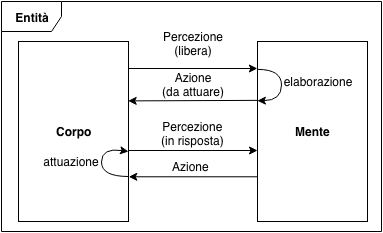
\includegraphics[width=8cm]{figures/Entita_struttura.png}
   \caption{Struttura di una generica entità}
   \label{entita_struttura}
\end{figure}

La figura \ref{entita_struttura} rappresenta la struttura di una generica entità, dove:

\begin{itemize}
   \item Il corpo esegue azioni e, in risposta a queste ultime, oppure, a seguito di determinati eventi esterni, trasmette le proprie percezioni alla mente.
   \item La mente elabora le percezioni per decidere quali azioni far svolgere al proprio corpo.
\end{itemize}




\section{Modelli computazionali}

In questo lavoro sono state utilizzate tecnologie con differenti modelli computazionali che
hanno portato a differenti soluzioni tecniche per effettuare una coerente integrazione dei sistemi utilizzati.
\marianiSays{ingrandirei anche la 2.3}
\subsection{Unity event loop}

Il modello computazionale presente su Unity è event loop: questo significa che tutti gli elementi presenti nella scena, come Script e GameObject, sono vincolati ad uno specifico lifecycle (raffigurato nell'immagine sottostante).
\begin{figure}[H]
   \centering
   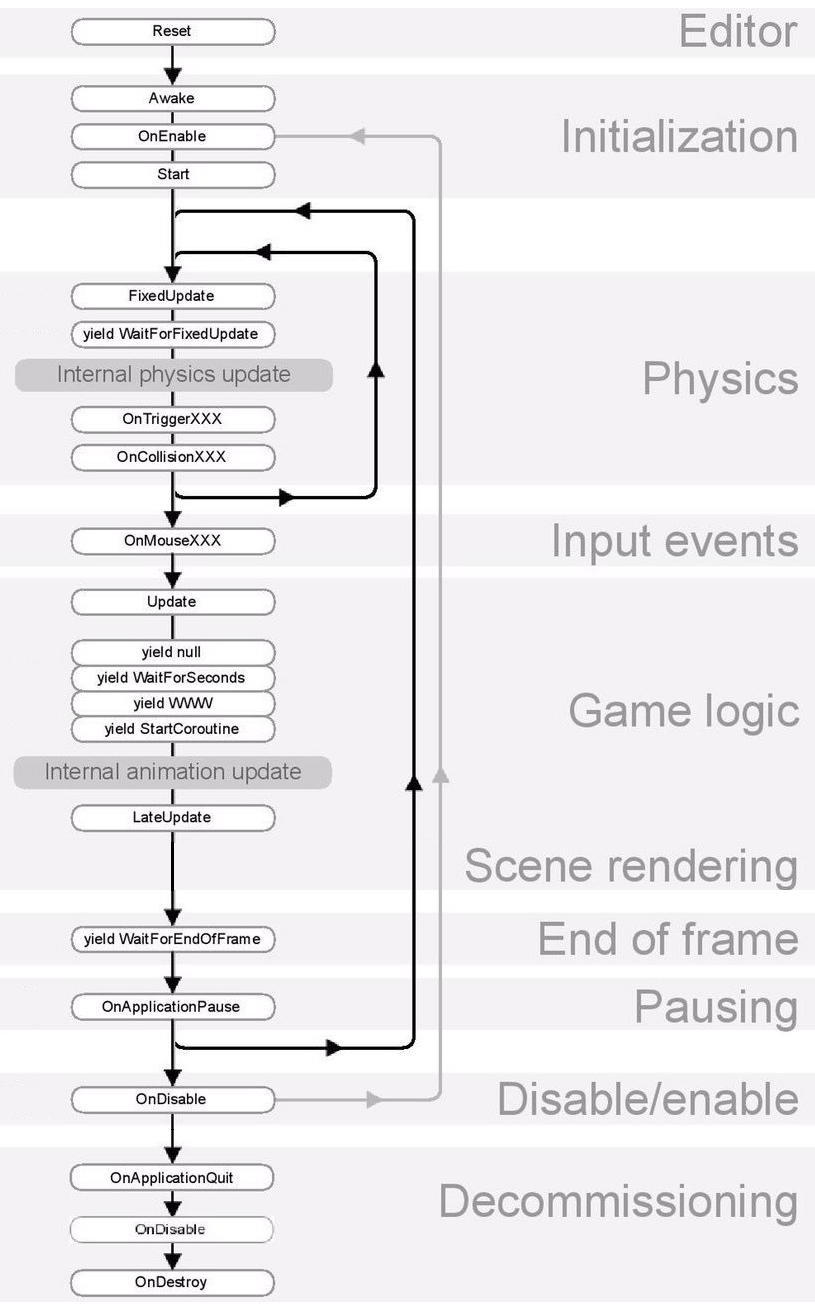
\includegraphics[height=\linewidth]{figures/Unity_lifecycle.jpeg}
   \caption{Unity lifecycle\cite{unity}}
\end{figure}

\improvement[inline]{Spiegare come ho fatto per notificare le "azioni" ai corpi}

Per interagire internamente tra i componenti, Unity mette disposizione delle API definite come "Event System"
con le quali è possibile inviare eventi agli oggetti nell'applicazione in base all'input, che si tratti di tastiera, mouse, tocco o input personalizzato.

Link utili:
\begin{itemize}
   \item \href{https://docs.unity3d.com/2018.3/Documentation/Manual/MessagingSystem.html}{Unity Messaging System}
   \item \href{https://docs.unity3d.com/2018.3/Documentation/Manual/MessagingSystem.html}{Unity Messaging System}: Utilizzato per generare eventi di ricezione nuovi messaggi direttamente inviati dalla WebSocket al VirtualBody invece di lasciare il VirtualBody a fare polling sulla coda dei messaggi in ingresso)
\end{itemize}

\subsection{Modello ad attori in Play}

\subsection{Jason BDI}

\subsection{CArtAgO}


\section{Architettura}

\begin{figure}[H]
   \centering
   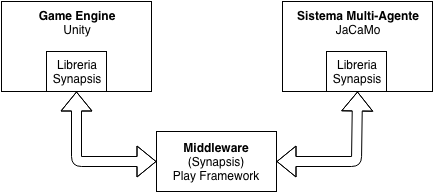
\includegraphics[width=\linewidth]{figures/Architettura_alto_livello.png}
   \caption{Architettura ad alto livello}
\end{figure}

L'immagine mostra la struttura del sistema realizzato per mettere in comunicazione MAS e GE attraverso l'introduzione di un middleware, realizzato con il framework Play, separato e autonomo rispetto alle differenti tecnologie utilzzate su MAS e GE.

\medskip

Per collegare al middleware i due sistemi, sono state realizzate due librerie, definite nell'immagine sovrastante "Libreria Synapsis", contenenti funzionalità di collegamento e comunicazione con Synapsis.
Le librerie rispettano astrazioni e modelli computazionali di entrambi i sistemi (MAS e GE) ed utilizzano la terminologia precedentemente elencata.

\begin{figure}[H]
   \centering
   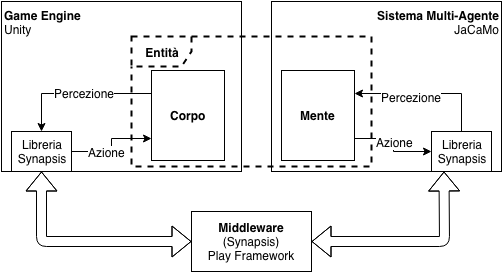
\includegraphics[width=\linewidth]{figures/Middleware_entity.png}
   \caption{Divisione di un'entità nel sistema}
\end{figure}

Aggiungendo un'entità alla struttura precedente è possibile notare come la stessa risulti suddivisa tra i due sistemi (MAS e GE) ed, attraverso il collegamento al middleware, venga reso possibile lo scambio di informazioni (percezioni, azioni) pur essendo computazionalmente separate.

\section{Struttura middleware} \label{struttura_middleware}

Synapsis è stato realizzato utilizzando il framework Play, illustrato nella sezione \ref{play}, le cui peculiarità sono la modularità e la distribuzione, raggiunte grazie all'utilizzo del sistema ad attori ed il modello computazionale associato: Event-driven/Message-driven. 

\medskip

Un sistema asincrono basato sui messaggi può utilizzare in modo più efficiente le risorse di un sistema poiché consuma risorse, come i thread, solo quando è effettivamente necessario. I messaggi possono essere recapitati anche a macchine remote (trasparenza della posizione), man mano che i messaggi vengono messi in coda e recapitati all'attore \cite{akka-book}.

\medskip

Il sistema ad attori ha portato alla definizione di un'entità "copia" all'interno del middleware, strutturata allo stesso modo dell'entità "esterna" presente in parte su GE ed in parte su MAS.

\medskip

Questa soluzione ha semplificato concettualmente la gestione delle entità esterne da parte del middleware. Difatti, realizzando rispettivamente un attore che identifica il corpo ed un attore che rappresenta la mente è venuta meno la realizzazione di una componente logica per lo smistamento dei messaggi ricevuti dall'esterno. Ad esempio, quando un attore "mente" riceve un messaggio dall'esterno è consapevole che tale messaggio è stato generato ed inviato dall'entità "mente" e, di conseguenza, è chiaro che il destinatario è l'attore "corpo", che a sua volta invia il messaggio all'entità "corpo" esterna.

\begin{figure}[H]
\centering
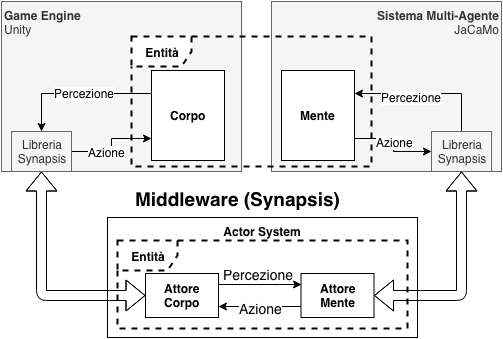
\includegraphics[width=\textwidth]{figures/Middleware_associazione_entita.png}
\caption{Associazione tra entità "esterna" ed "interna"}
\label{middleware_associazione_entita}
\end{figure}

Lo schema (figura \ref{middleware_associazione_entita}) illustra il concetto appena definito unito alla precedente architettura di sistema, dove ad ogni entità esistente nei sistemi MAS e GE viene associata una coppia di attori "mente" e "corpo" all'interno del middleware.



\chapter{Conclusioni}

Lo studio effettuato ha identificato le linee guida per collegare le astrazioni di Game Engine (GE) con quelle del Sistema Multi-Agente (MAS) con l'obiettivo di utilizzare la scena della GE come layer di modellazione dell'ambiente per il MAS. La definizione di un middleware (Synapsis) di collegamento ha permesso di non effettuare modifiche sostanziali sulle astrazioni dei due sistemi.

\medskip

I successivi passi comprenderanno la ricerca della tecnologia per realizzare il middleware, della tecnologia per collegare le tre componenti (GE, MAS, Synapsis) del sitema delineato e realizzare le librerie di supporto per GE e MAS, tenendo conto dei loro diversi modelli computazionali. 


\chapter{Caso di studio} \label{caso_studio}

Giunti a questo punto, si ha tutto il necessario per iniziare a considerare l’utilizzo del sistema per alcuni problemi reali. Il caso di studio in esame riguarda lo scenario dei "Recycling Robots", descritto nel seguito.

\section{Recycling Robots}

Come si può intuire dal nome, la scena contiene dei robot, i quali hanno il compito di riciclare la spazzatura presente nell'ambiente portandola nel rispettivo bidone. Il compito generale di un robot è divisibile in un ciclo di sotto-obiettivi, ad esempio:
\begin{enumerate}
    \item Cercare la spazzatura;
    \item Andare verso la spazzatura trovata;
    \item Prendere la spazzatura appena raggiunta;
    \item Cercare il bidone;
    \item Andare verso il bidone trovato;
    \item Riciclare la spazzatura.
\end{enumerate}

In questo particolare scenario è stato deciso di simulare la presenza di diversi tipi di spazzatura (plastica, vetro e carta) e, di conseguenza, sono stati creati diversi tipi di robot e bidoni.

\begin{figure}[H]
\centering
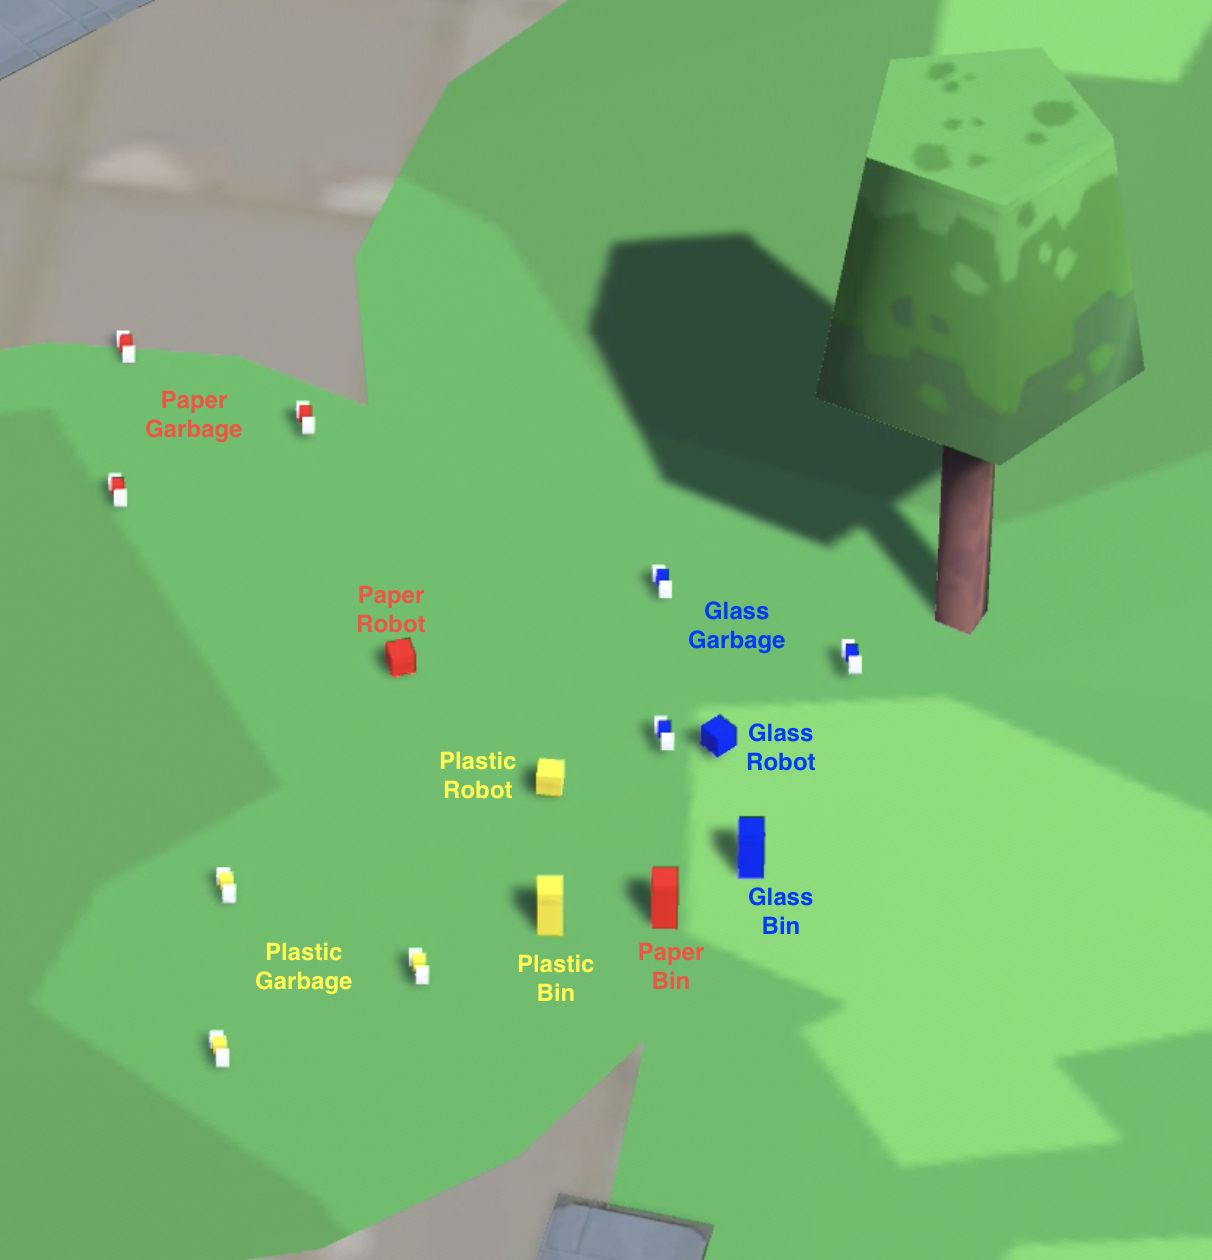
\includegraphics[width=\textwidth]{figures/recycling_robots.png}
\caption{Scenario Recycling Robots}
\label{scenario_recycling_robots}
\end{figure}

Ogni oggetto in scena è stato considerato come entità, con l'unica differenza che solo i robot sono dotati di autonomia attraverso un agente JASON ad essi collegato. La spazzatura ed i bidoni sono entità che, lato MAS, si fermano al concetto di artefatto. Per realizzare la scena è stato utilizzato WRLD \cite{wrld} che fornisce mappe 3D costruite usando dati geografici di alta qualità da poter utilizzare per la creazione di visualizzazioni 3D, esecuzione di simulazioni, o per lo sviluppo di giochi o esperienze dinamiche, basati sulla posizione geografica.

\subsection{Robot}

In questa sezione sono presenti i listati realizzati per definire il corpo e la mente dell'entità Robot.

\subsubsection{Corpo}

\lstinputlisting[label={robot},caption={Robot},language={[Sharp]C}]{code/Robot.cs}

Come da listato \ref{robot}, è stato realizzato uno script \textit{Robot}, che estende \textit{SynapsisBody}, il quale viene collegato al GameObject che rappresenta il robot nella scena Unity.
La presenza di API predefinite, all'interno di \textit{SynapsisBody}, ha ampiamente coperto tutte le attività che il robot deve svolgere in questo particolare scenario, difatti l'unica azione da definire è stata la colorazione del robot in base alla tipologia di spazzatura che è in grado di riciclare.

\subsubsection{Mente}

\lstinputlisting[label={robotArtifact},caption={Artefatto del robot},language={Java}]{code/RobotMind.java}

Il listato \ref{robotArtifact} definisce l'artefatto utilizzato nel MAS per collegarsi al middleware. Estendendo la classe \textit{SynapsisMind} è stato necessario definire una sola azione specifica che riguarda la colorazione del corpo del robot in base alla tipologia di spazzatura che lui è in grado di riciclare. 

\lstinputlisting[label={robotAgent},caption={Agente del robot},language={asl}]{code/robot.asl}

Il listato \ref{robotAgent} rappresenta l'agente JASON realizzato per definire l'automazione del robot. I beliefs iniziali sono utilizzati per definire il collegamento al middleware, mente il goal iniziale serve ad istanziare l'artefatto realizzato dell'immagine precedente \ref{robotArtifact}.

\medskip

Il plan \textit{synapsis\_counterpart\_status(Name, C)} è stato utilizzato per avviare l'obiettivo di "riciclare" del robot, mentre i successivi piani (\textit{stopped},\textit{found(Name)},\textit{arrived\_to(Name)}, \textit{picked(Name)}, \textit{released(Name)}) sono stati definiti per reagire alle percezioni inviabili dal corpo. I piani che iniziano per \textit{recycle} rappresentano tutte le fasi che il robot può utilizzare per riciclare la spazzatura.

\medskip

Nella parte finale del listato si può vedere in che modo è stata effettuata l'importazione dell'agente base presente nella libreria per JaCaMo.

\subsection{Bidone}

In questa sezione sono presenti i listati realizzati per definire il corpo e l'artefatto dell'entità Bidone.

\subsubsection{Corpo}

\lstinputlisting[label={bidone},caption={Script per il corpo del bidone},language={[Sharp]C}]{code/Bin.cs}

Come da listato \ref{bidone}, è stato realizzato un script \textit{Bin}, che estende \textit{SynapsisBody}, il quale viene collegato al GameObject che rappresenta il bidone nella scena Unity. L'unica azione da definire è stata la colorazione del GameObject "bidone" in base alla tipologia di spazzatura da lui accettata.

\subsubsection{Mente}

\lstinputlisting[label={binArtifact},caption={Artefatto del bidone},language={Java}]{code/BinMind.java}

Il listato \ref{binArtifact} definisce l'artefatto utilizzato nel MAS per collegarsi al middleware. Estendendo la classe \textit{SynapsisMind} è stato necessario definire una sola azione specifica che riguarda la colorazione del corpo del bidone in base alla tipologia di spazzatura da lui accettata. 

\subsection{Spazzatura}

In questa sezione sono presenti i listati realizzati per definire il corpo e l'artefatto dell'entità Spazzatura.

\subsubsection{Corpo}

\lstinputlisting[label={spazzatura},caption={Script per il corpo della spazzatura},language={[Sharp]C}]{code/Garbage.cs}

Come da listato \ref{spazzatura}, è stato realizzato uno script \textit{Garbage}, che estende \textit{SynapsisBody}, il quale viene collegato al GameObject che rappresenta la spazzatura nella scena Unity. Le azione da definire sono state la colorazione del GameObject "spazzatura" in base alla tipologia di spazzatura rappresentata e l'azione \textit{recycle\_me} per disattivare (riciclare) il GameObject dalla scena.

\medskip

Il metodo \textit{OnTransformParentChanged} viene utilizzato per sapere quando la spazzatura viene raccolta da un robot cosi da inviare la percezione \textit{picked\_up\_by} alla mente. Questa percezione viene utilizzata dal robot per capire quando è entrato in possesso della spazzatura che ha raggiunto.

\subsubsection{Mente}

\lstinputlisting[label={garbageArtifact},caption={Artefatto della spazzatura},language={Java}]{code/GarbageMind.java}

Il listato \ref{garbageArtifact} definisce l'artefatto utilizzato nel MAS per collegarsi al middleware. Estendendo la classe \textit{SynapsisMind} è stato necessario definire due azioni specifiche: la prima riguarda la colorazione del corpo della spazzatura in base alla tipologia di spazzatura rappresentata; mentre la seconda permette di riciclare sè stessa. L'ultima azione viene utilizzata dal robot dopo aver portato la spazzatura nel bidone corretto.

\subsection{Esempio interazione}

Viene ora illustrata l'interazione tra corpo e mente dell'entità robot durante la ricerca del bidone.

\begin{figure}[H]
\centering
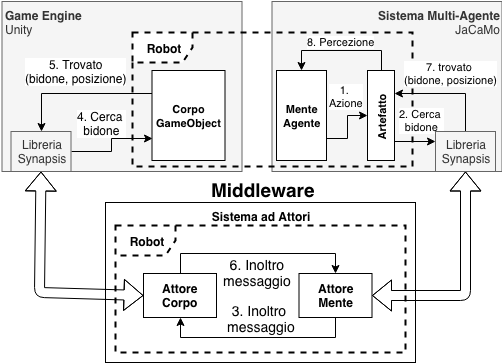
\includegraphics[width=\textwidth]{figures/scenario_esempio.png}
\caption{Esempio di comunicazione tra mente e corpo}
\label{scenario_esempio}
\end{figure}

L'immagine \ref{scenario_esempio} mostra il flusso ordinato di interazioni per l'esempio appena descritto. La mente per svolgere il plan \textit{"Cercare il bidone"} vuole inviare al proprio corpo l'azione \textit{"Cerca bidone"}. La richiesta di svolgere l'azione inizia dall'utilizzo dell'operazione presente nell'artefatto personale dell'agente\footnote{previa associazione dei due}, in possesso del canale per comunicare con il middleware.

\medskip

L'artefatto, quindi, invia il messaggio al middleware. L’attore "mente", presente nel middleware alla ricezione delle informazioni, inoltra le stesse all'attore "corpo", unico possessore del riferimento all’entità "corpo" presente su Unity in grado di inoltrare il messaggio al corpo "reale".  

\medskip

Alla ricezione del messaggio, l'entità corpo (GameObject) attua l'azione richiesta e risponde alla mente (Agente) inviandogli la percezione generata, ad esempio \textit{"trovato(nomeBidone)"}.

\medskip

A questo punto, la percezione viene mandata all'attore "corpo" nel middleware che, a sua volta, la inoltrerà all'attore "mente" e, di conseguenza, all'artefatto collegato. L'artefatto, nel momento in cui riceve la percezione, aggiunge quest'ultima alle sue proprietà osservabili che, automaticamente, aggiorneranno la BeliefBase dell'agente. 

\medskip

L'ultimo passaggio rappresenta il punto cruciale per completare il collegamento tra corpo e mente, dato che in questa maniera l'agente ha ricevuto la percezione dal proprio corpo. 

\subsubsection{Video dello scenario}

\'E possibile visualizzare lo scenario realizzato attraverso il video presente nel repository del middleware \ref{materiale_online}.

\chapter{Conclusioni e Sviluppi Futuri}

Il sistema sviluppato rappresenta un'implementazione preliminare di integrazione tra MAS e GE, e sfruttando le potenzialità offerte da Unity, si ha la conferma, ancora una volta, di come le due tecnologie – quella dei Game Engine e quella dei MAS – si sposino bene insieme. L'obiettivo primario di migliorare lo stato dell'arte dell'integrazione tra GE e MAS è stato raggiunto, mettendo a disposizione del programmatore un middleware e librerie per Unity e JaCaMo con le quali è possibile realizzare scenari relativamente complessi. Rimangono, tuttavia, margini di miglioramento e ulteriori studi da compiere.

\medskip

Per quanto riguarda il sistema nella sua interezza sarebbe interessante inserire SpatialTuples come mezzo abilitante la coordinazione, già utilizzato nei lavoro \cite{amslaurea16100} ed utilizzare il Web Socket Secure (WSS)\footnote{connessione criptata attraverso TLS/SSL} per migliorare la sicurezza complessiva delle comunicazioni. Sempre dal punto di vista della comunicazione sarebbe da aggiungere la possibilità di inviare strutture complesse (oggetti) nei parametri dei messaggi scambiati.

\medskip

Per quanto riguarda il middleware sarebbe sicuramente utile la realizzazione di una interfaccia grafica nella quale visualizzare le varie statistiche di invio e ricezione messaggi (raccolta delle tempistiche già presente), le entità presenti collegate, quali sono le entità mock, al fine di avere un vero e proprio centro di controllo del middleware.

\medskip 

In merito alla diffusione del sistema si potrebbero realizzare nuove librerie per aumentare l'estensione a più GE e/o MAS, cosi da non renderelo ad uso esclusivo di Unity e JaCamo ma, ad esempio, anche per altre GE (Unreal Engine, GameMaker, CryEngine) ed altri Multi-Agent System. A tal proposito si dovrebbbe aggiornare la libreria per JaCaMo supportandola alla sua ultima versione \href{https://sourceforge.net/projects/jacamo/files/version-0/}{JaCaMo 0.8}. 

\medskip 

Un altro interessante spunto di riflessione sui possibili lavori futuri riguarda la distribuzione: tutte le parti che compongono il sistema offrono diverse modalità di eseguire gli applicativi su diversi dispositivi. A tal proposito, Unity offre nativamente il supporto al Multiplayer che potrebbe essere sfruttato per indagare più a fondo in questa direzione.

\chapter*{Materiale online} \label{materiale_online}
\markboth{MATERIALE ONLINE}{}
\section*{Synapsis}
Repository con middleware e librerie disponibili all'indirizzo:\\
\href{https://gitlab.com/lucapascu/mas-ge-middleware}{https://gitlab.com/lucapascu/mas-ge-middleware}

\medskip

\section*{Progetto JaCaMo}
Repository con caso di studio e ambiente di test disponibili all'indirizzo:\\
\href{https://gitlab.com/lucapascu/mas-ge-jacamo}{https://gitlab.com/lucapascu/mas-ge-jacamo}

\medskip

\section*{Progetto Unity}
Repository con caso di studio e ambiente di test disponibili all'indirizzo:\\
\href{https://gitlab.com/lucapascu/mas-ge-jacamo}{https://gitlab.com/lucapascu/mas-ge-jacamo}


%----------------------------------------------------------------------------------------
%	THESIS CONTENT - APPENDICES
%----------------------------------------------------------------------------------------

\appendix % Cue to tell LaTeX that the following "chapters" are Appendices

% Include the appendices of the thesis as separate files from the Appendices folder
% Uncomment the lines as you write the Appendices

\chapter{Synapsis}

\section{Setup e Avvio}

Passi da seguire per configurare l'ambiente idoneo a Synapsis:
\begin{enumerate}
    \item Installare \href{https://www.scala-sbt.org/}{sbt};
    \item Scaricare il repository \textbf{mas-ge-middleware} utilizzando i link nella sezione \ref{materiale_online};
    \item Da terminale, navigare fino alla cartella \textbf{synapsis-middleware} interna al repository;
    \item Utilizzare il comando \textbf{sbt compile} per effettuare una prima compilazione del progetto.
\end{enumerate}

Passi da seguire per avviare Synapsis:
\begin{enumerate}
    \item Da terminale, navigare fino alla cartella \textbf{synapsis-middleware} interna al repository;
    \item Utilizzare il comando \textbf{sbt run} per avviare il progetto.
    \item Aprire un browser ed andare all'indirizzo \href{http://localhost:9000/}{http://localhost:9000/} per verificare l'effettivo avvio del progetto\footnote{La pagina principale è ancora un template senza funzionalità, serve solo a capire se il middleware è online}.
\end{enumerate}

\section{MockActor} \label{mock_actor}
Il MockActor è stato realizzato con l'obiettivo di velocizzare la fase di sviluppo, dato che permette di creare "finti" (dall'inglese "mock") attori che sostituiscono gli attori realmente collegati ad un'entità esterna. 

\medskip

Lo scenario ideale per l'utilizzo di questa modalità è quello di sviluppatori in grado di utilizzare solo una tecnologia, tra Unity e JaCaMo, e che attraverso la realizzazione di MockActor specifici riescano a sopperire alla necessità di uno sviluppo simultaneo.

\subsection{Come utilizzare il MockActor}

I passi da seguire per realizzare "finti" attori sono i seguenti:

\begin{enumerate}
    \item Creare una classe java che estenda MockActor,
    \item Posizionare la classe dentro il package \textbf{actor.mock} presente nel middleware,
    \item Implementare i metodi astratti come mostrato nel listato \ref{codiceMock}.
\end{enumerate}

\lstinputlisting[label={codiceMock},caption={Esempio di attore che estende la classe \textit{MockActor}},language=Java]{code/TestMock.java}

Il metodo \textit{parseIncomingMessage}, invocato ad ogni messaggio ricevuto dall'attore, permette allo sviluppatore di decidere come gestire tali messaggi che possono essere azioni o percezioni inviate dall'attore controparte e, quindi dall'entità esterna collegata al middleware.

\medskip

A disposizione dello sviluppatore sono presenti alcuni metodi, già implementati all'interno della classe \textit{MockActor}, per interagire con l'attore controparte (mente/corpo) e quindi con l'entità ad esso collegata. Il listato \ref{metodiMock} contiene tutti i metodi utilizzabili con i relativi commenti. 

\lstinputlisting[label={metodiMock},caption=Metodi per interagire con la controparte,language=Java]{code/MockActorAPI.java}

Il metodo \textit{sendResponse} è la condizione per inviare una generica risposta alla controparte e, quindi, utilizzabile per inviare un messaggio al corpo o alla mente. \'E da notare la presenza di interazioni predefinite dal punto di vista del contenuto del messaggio, difatti tutti i metodi che finiscono per \textit{Action} e per \textit{Perception} inseriscono automaticamente il contenuto principale del messaggio (sezione \ref{protocollo_messaggi}). Ad esempio, nel caso di \textit{searchAction} il contenuto sarà \textit{"search"}. L'obiettivo di questi metodi è quello di mettere subito a disposizione dello sviluppatore un primo set di Azioni e Percezioni già associate a una logica predefinita nelle restante parte del sistema.

\subsection{Architettura del sistema con MockActor}

Questa modalità di fast prototyping, modifica la architettura del sistema (Figure \ref{mock_actor_body} e \ref{mock_actor_mind}) in basa a quale tipologia di \textit{MockActor} viene utilizzato.

\begin{figure}[H]
\centering
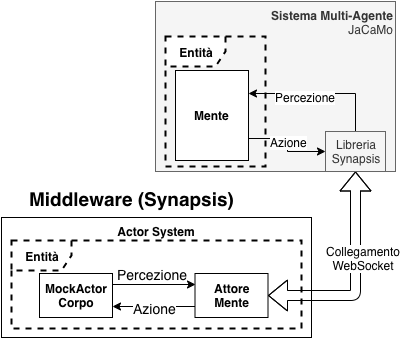
\includegraphics[width=0.6\textwidth]{figures/architettura_mock_actor_body.png}
\caption{Architettura con un MockActor di tipo \textit{body}}
\label{mock_actor_body}
\end{figure}

Con l'utilizzo di un "finto" attore che rappresenta la parte di entità "corpo" l'architettura del sistema si modifica di conseguenza, visto che viene meno la parte di Game Engine (GE). Le percezioni e le risposte alle azioni ricevute vengono simulate dal \textit{MockActor} di tipo "corpo" realizzato, che potrà essere successivamente sostituito dall'entità "corpo" in futuro realizzata sulla GE.

\begin{figure}[H]
\centering
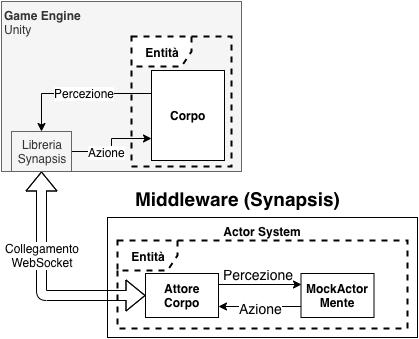
\includegraphics[width=0.6\textwidth]{figures/architettura_mock_actor_mind.png}
\caption{Architettura con un MockActor di tipo \textit{mind}}
\label{mock_actor_mind}
\end{figure}

Con l'utilizzo di un "finto" attore che rappresenta la parte di entità "mente", l'architettura del sistema si modifica di conseguenza, visto che viene meno la parte di Sistema Multi-Agente (MAS). L'autonomia viene simulata dal \textit{MockActor} di tipo "mente" realizzato che potrà essere successivamente sostituito dall'entità "mente" realizzata sul MAS.

\subsection{Istanziare MockActor}

\subsubsection{Istanziare dall'interno del middleware}

Lo sviluppatore ha a disposizione due metodi all'interno della classe \textbf{Application}, che permettono di istanziare uno o più "finti" attori precedentemente realizzati.

\lstinputlisting[label={mockactorapplication},caption={Metodi per istanziare un MockActor nel middleware},language=Java]{code/Application_mock.java}

I metodi \textit{spawnMockActor} e \textit{spawnMockActors} permettono di creare, all'interno del sistema, generici attori dato che accettano classi Java che estendano la classe \textit{MockActor}. Questi metodi, come da listato \ref{mockactorapplication}, vanno utilizzati nel costruttore della classe \textbf{Application} per essere certi di istanziare gli attori all'avvio dell'applicazione.

\subsubsection{Istanziare dall'esterno del middleware}

Per istanziare MockActor runtime sono state fornite delle API nelle rispettive librerie di JaCaMo e Unity che comunicano direttamente con il middleware e permettono la creazione di questi attori attraverso l'invio di un messaggio predefinito.

\medskip

Su Unity è stato realizzato un processo che utilizza l'interfaccia grafica dell'IDE (figura \ref{gui_script}). Collegando al GameObject uno script che estende \textit{SynapsisBody} si ottiene il seguente risultato:

\begin{figure}[H]
\centering
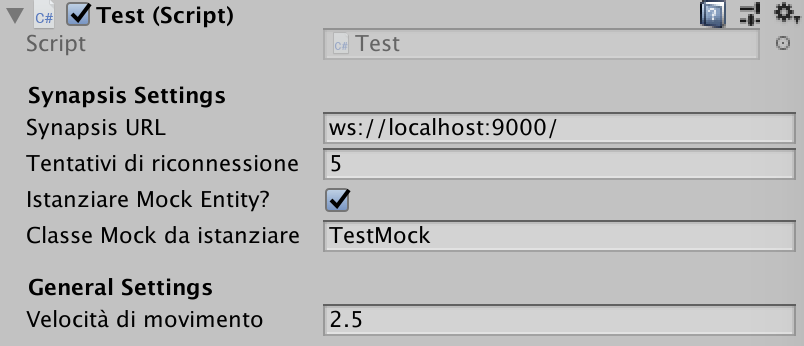
\includegraphics[width=0.7\textwidth]{figures/Unity_Test_editor.png}
\caption{Interfaccia grafica di gestione dello script}
\label{gui_script}
\end{figure}

I parametri \textit{"Istanziare Mock Entity?"} e \textit{"Classe Mock da istanziare"}, permettono al GameObject di creare il messaggio da inviare al middleware appena stabilito il collegamento WebSocket.

\medskip

Per JaCaMo sono presenti due modalità. La prima è effettuabile attraverso l'invocazione di uno specifico metodo presente nell'artefatto \textit{SynapsisMind}.

\lstinputlisting[caption={Metodo per istanziare MockActor dall'artefatto},language=Java]{code/SynapsisMind_istanziare_mock_actor.java}

La seconda utilizza uno specifico plan presente nell'agente \textit{SynapsisBaseAgent} che a loro volta utilizza l'operazione (metodo) del listato precedente.

\lstinputlisting[caption={Piano per istanziare MockActor},language=asl]{code/plan_mock_actor.asl}

In entrambe le situazioni, lo sviluppatore deve fare attenzione a scrivere correttamente il nome della classe da istanziare ed a posizionare la classe Java nel corretto package (actors.mock).



\subsection{JaCaMo}

JaCaMo è un framework per la programmazione orientata agli agenti che combina tre tecnologie già affermate e sviluppate da diversi anni.

\medskip

Un sistema multi-agente JaCaMo o, equivalentemente, un sistema software programmato con JaCaMo è definito da un'organizzazione Moise di agenti BDI autonomi basati su concetti come ruoli, gruppi, missione e schemi, implementati tramite Jason, che lavorano in ambienti condivisi distribuiti basati su artefatti, programmati in CArtAgO.

\medskip

Ognuna delle tre tecnologie indipendenti che compongono il framework ha il proprio set di astrazioni, modelli di programmazione e meta-modelli di riferimento, per questo motivo in JaCaMo è stato realizzato un meta-modello globale, con l'obiettivo di definire le dipendenze, connessioni, mapping concettuali e le sinergie tra le differenti astrazioni rese disponibili da ogni livello \cite{BOISSIER2013747}.

\begin{figure}[H]
\centering
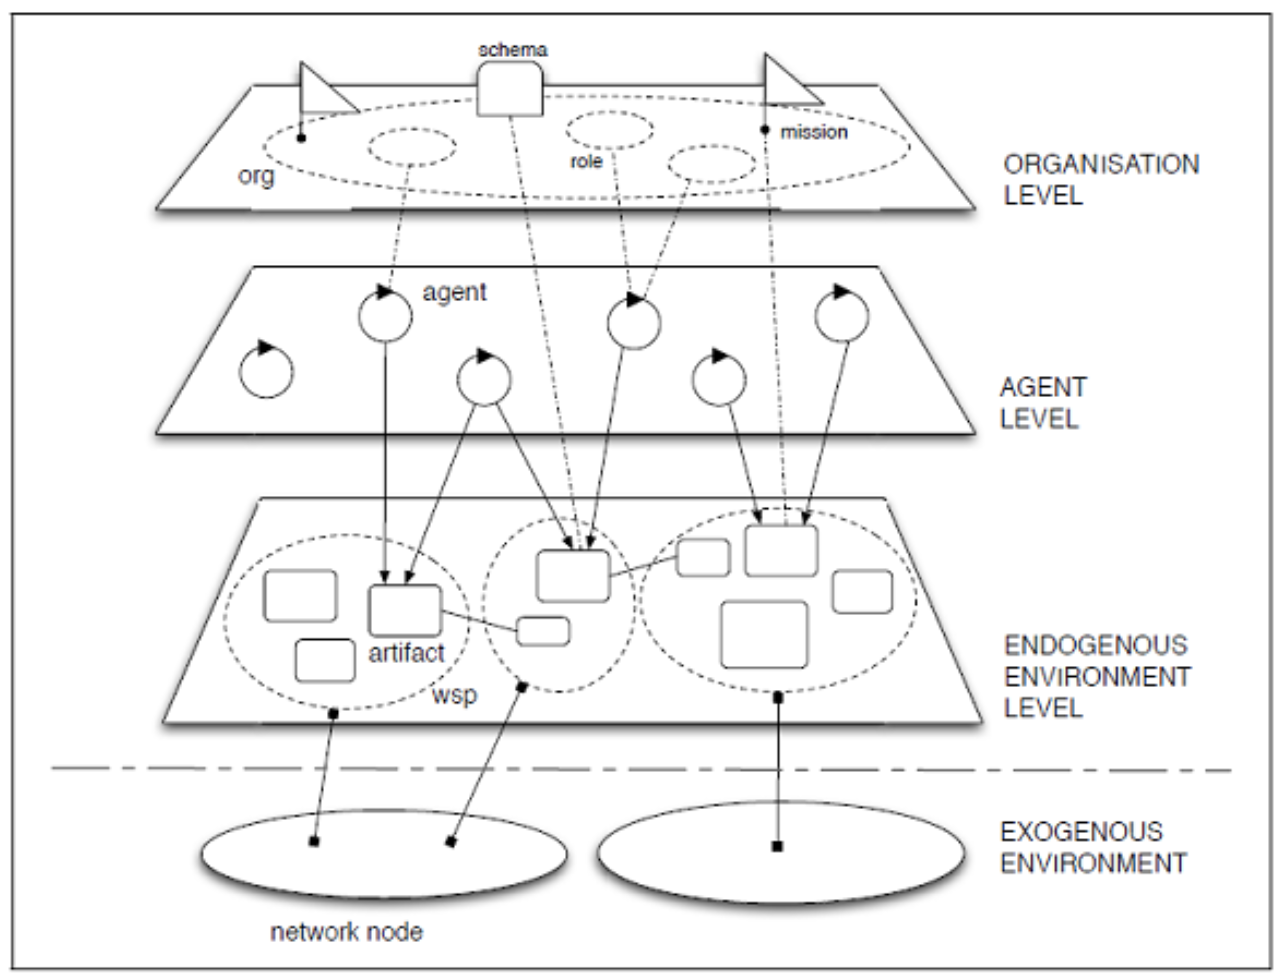
\includegraphics[width=\textwidth]{figures/JaCaMo_levels.png}
\caption{Livelli che compongono il framework JaCaMo \cite{BOISSIER2013747}}
\label{livelli_jacamo}
\end{figure}

\subsubsection{Jason} \label{jason}

Jason è un interprete di AgentSpeak che implementa la semantica operazionale del linguaggio e fornisce una piattaforma di sviluppo per Sistemi Multi-Agente, con molte funzionalità personalizzabili dall'utente.

\medskip

Le astrazioni appartenenti alla dimensione degli agenti, correlate al meta-modello Jason, sono principalmente ispirate all'architettura BDI sulla quale Jason è radicato. Quindi un agente è un'entità composta da un insieme di "beliefs", che rappresenta lo stato corrente e la conoscenza dell'agente sull'ambiente in cui si trova, una serie di "goals", che corrispondono a compiti che l'agente deve perseguire e una serie di "plans" ossia sequenze di azioni (external action or internal action), innescate da eventi, che gli agenti possono comporre, istanziare ed eseguire dinamicamente per compiere i "goals" \cite{jason-book}.

\subsubsection{CArtAgo}
Per quanto riguarda l'ambiente, ciascuna istanza dell'ambiente CArtAgO\footnote{Common ARTifact infrastructure for AGents Open environments} è composta da una o più entità workspace. Ogni workspace è formato da un insieme di artefatti, che forniscono un insieme di operazioni e proprietà osservabili, definendo anche l'interfaccia di utilizzo degli artefatti. L'esecuzione dell'operazione potrebbe generare aggiornamenti delle proprietà osservabili e degli eventi osservabili specifici. L'ultima entità relativa all'ambiente è il “manual”, un'entità utilizzata per descrivere le funzionalità fornite da un artefatto.
Cartago è basato sul meta-modello A\&A (Agents \& Artifacts), che definisce gli agenti come entità computazionali che compiono qualche tipo di attività che mira a uno scopo e gli artefatti come risorse e strumenti costruiti dinamicamente, usati e manipolati dagli agenti per supportare/realizzare le loro attività \cite{cartago}.

\smallskip

\paragraph{Artefatto}
L'artefatto è un'entità reattiva, non autonoma, stateful, riutilizzabile, controllabile ed osservabile. Modellano strumenti, risorse e porzioni di ambiente agendo da strumenti mediatori di azioni e interazioni sociali tra partecipanti individuali e lo stesso ambiente \cite{Omicini2008}.

\begin{figure}[H]
\centering
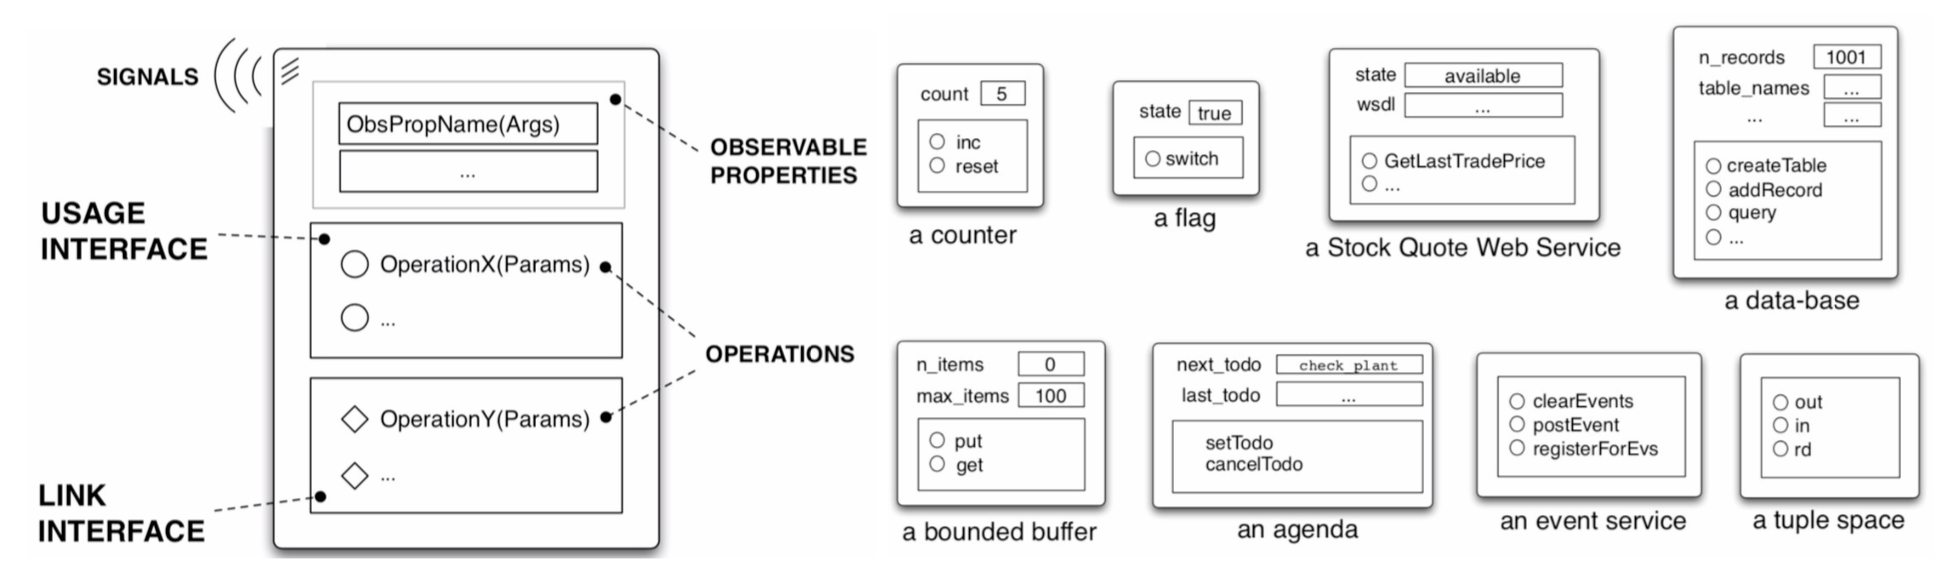
\includegraphics[width=\linewidth]{figures/Artifact_structure_example.png}
\caption{Struttura artefatto con relativi esempi}
\end{figure}

La modalità di interazione tra artefatto ed agente viene riepilogato nell'immagine sottostante.

\begin{figure}[H]
\centering
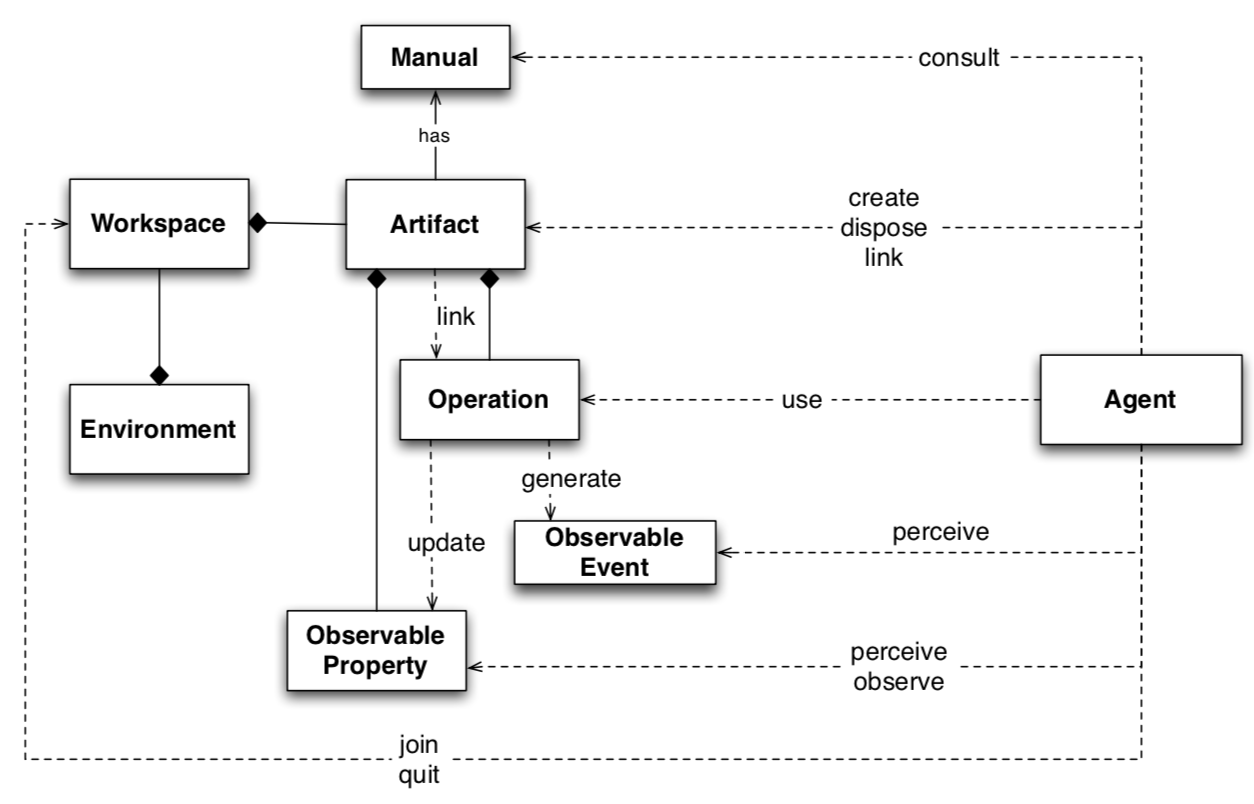
\includegraphics[width=\linewidth]{figures/Artifact_Agent_interaction.png}
\caption{Interazione tra agente ed artefatto}
\end{figure}

\subsubsection{Moise}
Moise è un meta-modello organizzativo per MAS basato sulle nozioni di ruoli, gruppi e missioni. Abilita un MAS ad avere specifiche esplicite per la sua organizzazione. Queste specifiche sono usate sia dagli agenti per ragioni inerenti la loro organizzazione, sia da una piattaforma organizzativa che si assicuri che gli agenti seguano le specifiche.

Moise permette di definire una gerarchia di ruoli con autorizzazioni e missioni, da assegnare agli agenti. Questo permette ai sistemi con un'organizzazione forte, di guadagnare proprietà di apertura (essenzialmente, la proprietà di lavorare con un numero e una diversità di componenti che non è imposta una volta per tutte) e adattamento.

\chapter{Unity} \label{appendice_Unity}

\section{Utilizzare la libreria}

La distribuzione della libreria realizzata per Unity viene effettuata attraverso la generazione di un \textit{Asset packages} ossia collezione di file e dati, realizzati da progetti Unity, compressi e memorizzati in un unico file, simile ad una cartella compressa. 
All'interno del package, la struttura dei file e i metadati rimangono gli stessi dell'originale così da rendere possibile la distribuzione del codice sorgente e delle dipendenze esterne.

\medskip

La libreria prodotta, \textit{Synapsis.unitypackage}, è disponibile sul repository del middleware (sezione \ref{materiale_online}) e per importarla è necessario creare un nuovo progetto Unity, da menu "Assets"->"Import Package"->"Custom Package" e selezionare la libreria.


\section{Realizzare Script custom}

Come spiegato nella sezione \ref{libreria_unity}, la classe \textit{SynapsisBody} è uno script che contiene le funzionalità di collegamento al middleware. Per realizzare uno script custom è sufficiente creare una nuova classe che estenda \textit{SynapsisBody}.

\lstinputlisting[caption=Esempio di script che estende SynapsisBody,language={[Sharp]C}]{code/Test.cs}

I metodi \textit{CounterpartEntityReady} e \textit{CounterpartEntityUnready} vengono utilizzati per conoscere lo stato di collegamento con la controparte mente. Questi metodi vengono automaticamente invocati in base alle informazioni ricevute dal middleware.

\medskip

Collegando lo script sopra elencato al GameObject compaiono, nella sezione "Inspector" di Unity", le configurazioni necessarie per definire il collegamento al middleware, nell'editor di Unity.

\begin{figure}[H]
\centering
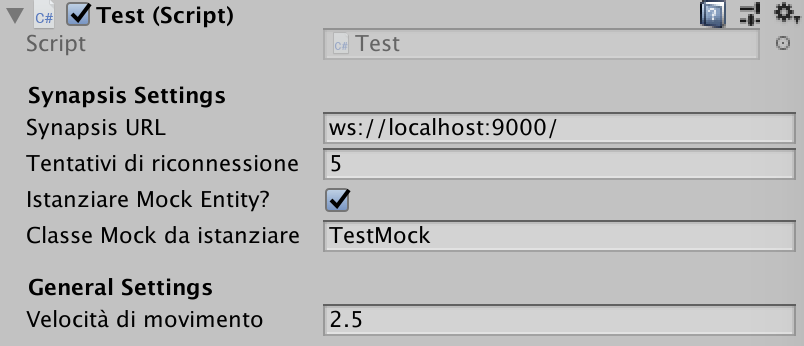
\includegraphics[width=\textwidth]{figures/Unity_Test_editor.png}
\caption{Configurazioni dello Script Test che estende SynapsisBody}
\end{figure}

Le configurazioni riguardano il collegamento al middleware, la necessità di instanziare una MockEntity e la velocità di movimento dell'entità (se deve effettuare spostamenti nell'ambiente).

\chapter*{Ringraziamenti}
\markboth{RINGRAZIAMENTI}{}

\noindent Giunto alla conclusione di questo cammino, mi trovo in difficoltà a scrivere i ringraziamenti...

\medskip

\noindent Il motivo è semplice, vorrei ringraziare uno per volta tutte le persone conosciute in questi anni e dirgli come hanno contribuito a farmi diventare la persona che sono ora ma questa paginetta non sarà sufficiente. Tranquilli ho una soluzione anche per voi!

\medskip

\noindent Ale e Filo, siete le prime persone con le quali sia riuscito a creare una squadra di smanettoni, grazie per avermi insegnato che la taverna di casa è un ottimo posto per costruire App e robot in compagnia. \#RepairCityTornerà

\medskip 

\noindent UniboMotorsport, il Team che mi ha completamente stravolto le ultime cinque estati (per fortuna solo quelle). Assieme a voi ho riscoperto la mia passione per il Motorsport, dalla convergenza, allo stare a sedere ore in macchina per creare un sedile, e sopratutto al vivere di redbull per reggere le fatiche di trasferte infinite. Abbiamo girato gran parte dell'Europa, pure il Brasile (che matti), ma mai mi scorderò di voi e di Collamarini, il luogo dove tutto prendeva forma. \#KeepPushing

\medskip 

\noindent Marco e Scat, il duo del dormire in camper al contrario (ingegneri si nasce). Con voi ho passato i più bei momenti della FSAE e devo ammettere che si è creata un'amicizia speciale (a base di pappardelle al cinghiale) a cui tengo e che continuerò a coltivare con molto piacere. \#QuelliDelRotax

\medskip

\noindent Noemi, l'unica persona in grado di cambiarmi la giornata, dire grazie è riduttivo <3. Sei riuscita a fare la tua tesi e nello stesso tempo aiutarmi a correggere questa (migliorerò l'utilizzo degli apostrofi). Oggi siamo ad 1 anno e 250 giorni, come minimo ne voglio altrettanti \#C'èQualcosaDiGrande \#IlTuoPesarese 

\medskip

\noindent Family (Lucky ovviamente incluso), siete stati la fonte di energia di tutto questo, grazie per avermi supportato e soprattutto sopportato. \#GrazieDiTutto \#ReLucky

\medskip

\noindent Mariani e Omicini, incredibilmente motivanti, mi avete dato una carica (e mano) pazzesca lungo tutto questo ultimo sprint. \#ProfDelFuturo

\medskip

\noindent Come detto in precedenza non riesco a ringraziare tutti, ma una cosa la posso fare: chiunque si senta escluso è libero di autoinvitarsi ovunque io sia e chiedermi di offrirgli una "pizza" (sappiamo tutti quale intendo) ed io sarò lieto di metterci pure la maionese sopra (un po' come se fosse la mia firma).\#UnaRossinièpersempre 


%%%%%%%%%%%%%%%%%%%%%%%%%
% inizio parte finale del documento
%
% eventuali appendici, bibliografia obbligatoria,
% eventuale lista delle tabelle e delle figure
%%%%%%%%%%%%%%%%%%%%%%%%%
\backmatter

%\listoftodos[Lista Note]
\listoffigures
%\listoftables
\lstlistoflistings
\bibliography{biblio}
\bibliographystyle{abbrv}

% chiusura del documento
\end{document}
